%\documentclass[10pt,landscape,a4paper]{article}
\documentclass[10pt,landscape,letterpaper]{article}
\usepackage{multicol}
\usepackage{calc}
\usepackage{ifthen}
\usepackage[landscape]{geometry}
\usepackage{listings}
\usepackage{graphicx}
\usepackage{cclicenses}
\usepackage[T1]{fontenc}
\usepackage[scaled]{beramono}

% This sets page margins to .5 inch if using letter paper, and to 1cm
% if using A4 paper. (This probably isn't strictly necessary.)
% If using another size paper, use default 1cm margins.
\ifthenelse{\lengthtest { \paperwidth = 11in}}
           { \geometry{top=.5in,left=.5in,right=.5in,bottom=.5in} }
           {\ifthenelse{ \lengthtest{ \paperwidth = 297mm}}
             {\geometry{top=1cm,left=1cm,right=1cm,bottom=1cm} }
             {\geometry{top=1cm,left=1cm,right=1cm,bottom=1cm} }
           }

% Turn off header and footer
\pagestyle{empty}

% Redefine section commands to use less space
\makeatletter
\renewcommand{\section}{\@startsection{section}{1}{0mm}%
                                {-1ex plus -.5ex minus -.2ex}%
                                {0.5ex plus .2ex}%x
                                {\normalfont\large\bfseries}}
\renewcommand{\subsection}{\@startsection{subsection}{2}{0mm}%
                                {-1explus -.5ex minus -.2ex}%
                                {0.5ex plus .2ex}%
                                {\normalfont\normalsize\bfseries}}
\renewcommand{\subsubsection}{\@startsection{subsubsection}{3}{0mm}%
                                {-1ex plus -.5ex minus -.2ex}%
                                {1ex plus .2ex}%
                                {\normalfont\small\bfseries}}
\makeatother

% Don't print section numbers
\setcounter{secnumdepth}{2}
\setlength{\parindent}{0pt}
\setlength{\parskip}{0pt plus 0.5ex}

\lstdefinelanguage{aadl}
{morekeywords={in,out,package,end,bus,data,thread,port,group,process,processor,
system,memory,device,subprogram,classifier,public,connection,private,event,property,set,applies,to,
units,type,implementation,parameter,reference},
  morekeywords={properties,feature, features,annex,modes,connections,flows,
  subcomponents,calls,binding, with, extends, is, renames, all, requires, provides, access, inherit, list, of,virtual},
  morekeywords={aadlinteger,aadlboolean,aadlstring,aadlfloat},
morecomment=[l]{--},
basicstyle=\ttfamily,
}

% ------------------------------------------------------------------------------

\begin{document}

\raggedright
\footnotesize
\begin{multicols}{3}
\setlength{\premulticols}{1pt}
\setlength{\postmulticols}{1pt}
\setlength{\multicolsep}{1pt}
\setlength{\columnsep}{2pt}

\begin{center}
  \Large{\textbf{AADLv2 Cheat Sheet: Basics}} \\
  \rule{0.3\linewidth}{0.25pt}
\end{center}

%-------------------------------------------------------------------------------
\section{AADL Components}

\subsection{Taxonomy of model elements}

\begin{tabular}{@{}ll@{}}
\verb!component category!       & class: e.g. thread, data, \ldots\\
\verb!component type!           & features, flows, properties.\\
\verb!component implementation! & subcomponents, connections\\
                                & call sequence, flow impl.\\
                                & and properties.\\
\verb!packages!                 & Namespace for components.\\
\verb!property sets!            & Non-functional properties.\\
\end{tabular}

\subsection{Component categories}

\begin{tabular}{@{}ll@{}}
\verb!data!       & data type\\
\verb!thread!           & execution flow\\
\verb!thread group! & group of threads\\
\verb!subprogram! & sequential flow\\
\verb!process! & address space\\
\verb!memory!& storage area\\
\verb!bus!& physical interconnect\\
\verb!processor!& execution resource\\
\verb!device!& I/O\\
\verb!virtual processor!& partition \\
\verb!virtual bus!& logical interconnect\\
\verb!system!& encapsulation block\\
\verb!abstract!& component template\\
\end{tabular}

\subsection{Component type declaration}

{\scriptsize
\begin{lstlisting}[language=aadl]
<component_category> <component_identifier>
     extends <component_type_identifier'>
features
   -- some features
properties
   -- some properties
end <component_identifier>;
\end{lstlisting}
}

\begin{tabular}{@{}ll@{}}
\verb!extends! & inherit from another component type.\\
\verb!features! & list ports, access to other elements.\\
\verb!properties! & NFP properties for this type.\\
\end{tabular}

\subsection{Component implementation declaration}

{\scriptsize
\begin{lstlisting}[language=aadl]
<component_category> implementation
 <component_identifier>
   extends <component_implementation_identifier'>
subcomponents
   --
calls
   -- some call sequences
connections
   --
properties
   -- some properties
flows
modes
end <component_identifier>;
\end{lstlisting}
}

\begin{tabular}{@{}ll@{}}
\verb!subcomponents! & subcomponents (internals)\\
\verb!extends! & inherit from another component type.\\
\verb!calls! & call sequence (only thread and subprograms)\\
\verb!connections! & link subcomponents\\
\verb!properties! & NFP properties for this type.\\
\verb!flows! & flow implementation\\
\verb!modes! & mode automata\\
\end{tabular}

\subsection{Packages}

{\scriptsize
\begin{lstlisting}[language=aadl]
package <package_identifier>
public
   with <package_identifier_1>;
   renames <package_idenfier_1>::all;
   --  imports all entities
   renames <package_idenfier_1>::Id;
   --  partial import
   Id2 renames <package_idenfier_1>::Id2;
   --  partial renaming
end <package_identifier>;
\end{lstlisting}
}

\begin{tabular}{@{}ll@{}}
\verb!with! & import entities\\
\verb!public! & all entities are visible, need qualification\\
\verb!private! & hide implementation\\
\verb!renames! & full import, no qualification\\
\end{tabular}

\subsection{Component Features}

\begin{tabular}{@{}ll@{}}
\verb!data port! & unqueued information\\
\verb!event (data) port! & pure or type signal, queued \\
\verb!port direction!& in (reception), out (emission), in out\\
\verb!requires access! & need to access a data or spg\\
\verb!provides access!&\\
\end{tabular}

\subsection{Features connections}

Connections are directional:
{\scriptsize
\begin{lstlisting}[language=aadl]
connections
  parameter <parameter_out> -> <parameter_in>
  port <port_out> -> <port_in>
  access <provider> -> <requirer>
\end{lstlisting}
}

\section{AADL Properties}

\subsection{Property sets}

{\scriptsize
\begin{lstlisting}[language=aadl]
property set <ps_identifier>
  -- ...
end <ps_identifier>;
\end{lstlisting}
}

\subsection{Pre-defined property sets:}

\begin{tabular}{@{}ll@{}}
\verb!deployment_properties! & binding constraints\\
\verb!thread_properties! & dispatching, concurrency, \ldots \\
\verb!timing_properties!& support of time\\
\verb!communication_properties! & communication mechanisms\\
\verb!memory_properties! & use of storage areas\\
\verb!programming_properties! & link to implementation\\
\verb!modeling_properties! & name resolution rules\\
\verb!aadl_project! & project-specific constants\\
\end{tabular}

% XXX inherit

\subsection{deployment\_properties}

{\scriptsize
\begin{lstlisting}[language=aadl]
property set Deployment_Properties is
  Actual_Processor_Binding:
   inherit list of reference
    (processor, virtual processor)
  applies to (thread, thread group, process,
   system, virtual processor, device);
  --  Binding components to a processor

  Actual_Memory_Binding:
        inherit list of reference (memory)
  applies to (thread, thread group,
   process, system, processor, device, data,
   data port, event data port, feature group,
   subprogram);
  --  Binding components to a memory

  Actual_Connection_Binding:
   inherit list of reference (processor,
    virtual processor, bus,
    virtual bus, device, memory)
   applies to (port, connection, thread group,
    process, system, virtual bus);
  --  Binding components to a connection

  Scheduling_Protocol: inherit list of
   Supported_Scheduling_Protocols
    applies to (virtual processor, processor);
  --  See aadl_project for a full list
end Deployment_Properties;
\end{lstlisting}
}
\subsection{thread\_properties}

{\scriptsize
\begin{lstlisting}[language=aadl]
property set Thread_Properties is
  Dispatch_Protocol: Supported_Dispatch_Protocols
   applies to (thread);
  -- Periodic, Sporadic, Aperiodic, Timed,
  -- Hybrid, Background

  Priority: inherit aadlinteger
   applies to (thread, thread group,
    process, system, device, data);

  Concurrency_Control_Protocol:
   Supported_Concurrency_Control_Protocols
    applies to (data);
end Thread_Properties;
\end{lstlisting}
}

\subsection{timing\_properties}

{\scriptsize
\begin{lstlisting}[language=aadl]
property set Timing_Properties is
  Time: type aadlinteger 0 ps .. Max_Time
    units Time_Units;
  Time_Range: type range of Time;

  Compute_Deadline: Time
   applies to (thread, device, subprogram,
    event port, event data port);
  --  Deadline of an activity

  Compute_Execution_Time: Time_Range
   applies to (thread, device, subprogram,
    event port, event data port);
  --  Worst Case Execution Time

  Period: inherit Time
   applies to (thread, thread group,
    process, system, device);

 Timing: enumeration
  (sampled, immediate, delayed)
   => sampled applies to (port);
 --  Timing of communications
end Timing_Properties;
\end{lstlisting}
}

\subsection{communication\_properties}

{\scriptsize
\begin{lstlisting}[language=aadl]
property set Communication_Properties is
  Overflow_Handling_Protocol: enumeration
    (DropOldest, DropNewest, Error)
   => DropOldest
  applies to (event port,
   event data port, subprogram);

  Queue_Processing_Protocol:
   Supported_Queue_Processing_Protocol => FIFO
   applies to (event port,
    event data port, subprogram);

  Queue_Size: aadlinteger 0 .. Max_Queue_Size => 1
   applies to (event port,
    event data port, subprogram);
end Communication_Properties;
\end{lstlisting}
}
\subsection{programming\_properties}

{\scriptsize
\begin{lstlisting}[language=aadl]
property set Programming_Properties is
  Compute_Entrypoint:
   classifier (subprogram classifier)
  applies to (thread,
   subprogram, event port, event data port);
 --  Also Initialize_, Recovery_, ..

 Source_Language: inherit
  Supported_Source_Languages
   applies to (subprogram, data,
    thread, thread group, process, system,
    bus, virtual bus, device, processor);

 Source_Text: inherit list of aadlstring
  applies to (data, port,
   virtual bus, subprogram, thread,
   thread group, process, system,
   memory, bus, device, processor,
   parameter, feature group, package);
end Programming_Properties;
\end{lstlisting}
}


\section{Graphical AADL notations}

\begin{center}
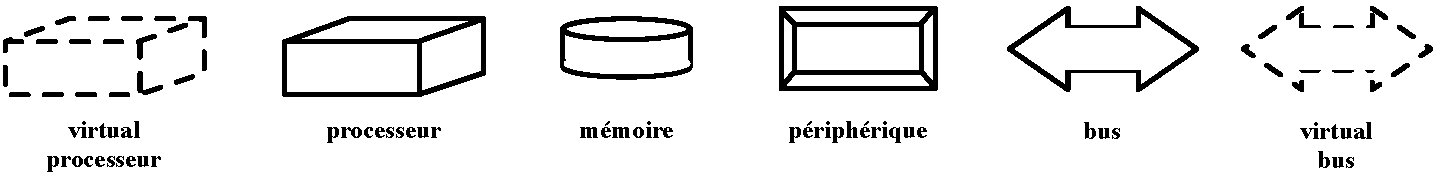
\includegraphics[width=.25\textwidth]{aadl-lang-hard.pdf}
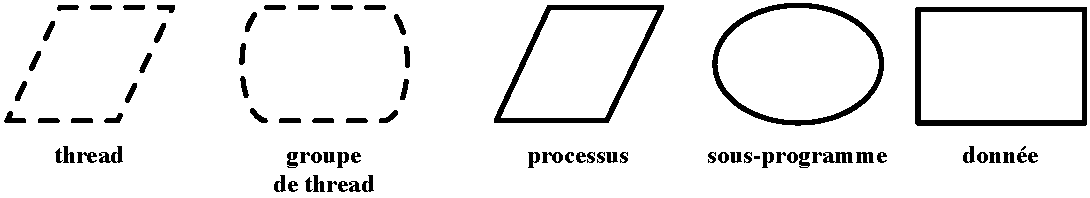
\includegraphics[width=.25\textwidth]{aadl-lang-soft.pdf}
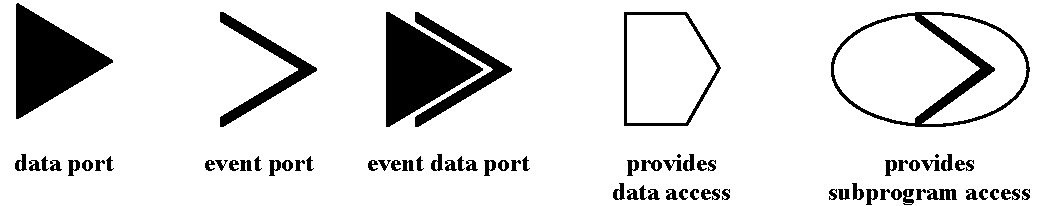
\includegraphics[width=.25\textwidth]{aadl-lang-itf.pdf}
\end{center}

\section{Example: Producer/Consumer}

This models proposes a simple producer/consumer pattern, covering
most AADLv2 constructs from this sheet.

\begin{center}
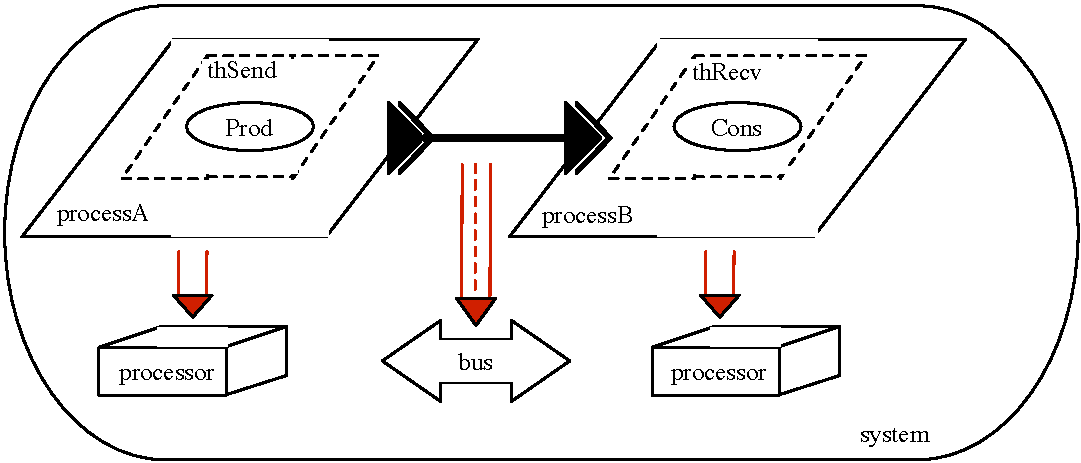
\includegraphics[width=.25\textwidth]{aadl-lang-example.pdf}
\end{center}

{\scriptsize
\begin{lstlisting}[language=aadl]
package Software
public
 with Data_Model;

 data Simple_Type
 properties
  Data_Model::Data_Representation => integer;
 end Simple_Type;

 subprogram Do_Ping_Spg
 features
  Data_Source : out parameter Simple_Type;
 end Do_Ping_Spg;

 subprogram Ping_Spg
 features
  Data_Sink : in parameter Simple_Type;
 end Ping_Spg;

 thread thSend
 features
  Data_Source : out event data port Simple_Type;
 end thSend;

 thread implementation thSend.Impl
 calls
  Mycall : { P_Spg : subprogram Do_Ping_Spg; };
 connections
  parameter P_Spg.Data_Source -> Data_Source;
 properties
  Dispatch_Protocol => Periodic;
  Period            => 1000 ms;
  Priority          => 2;
 end thSend.Impl;

 thread thRecv
 features
  Data_Sink : in event data port Simple_Type;
 end thRecv;

 thread implementation thRecv.Impl
 connections
   parameter Data_Sink -> Q_Spg.Data_Sink;
 properties
   Dispatch_Protocol  => Sporadic;
   Period             => 10 ms; -- MIAT
   Priority           => 1;
   Compute_Entrypoint => classifier (Ping_Spg);
 end thRecv.Impl;
end Software;

package PING_Package
public
 with software;
 with deployment;

 processor the_processor
 features
  ETH : requires bus access Ethernet_Bus;
properties
  Scheduling_Protocol =>
   POSIX_1003_HIGHEST_PRIORITY_FIRST_PROTOCOL;
 end the_processor;

 bus Ethernet_Bus end Ethernet_Bus;

 process A
 features
  Out_Port : out event data port Software::Simple_Type;
 end A;

 process implementation A.Impl
 subcomponents
   Pinger        : thread Software::thSend.Impl;
 connections
   port Pinger.Data_Source -> Out_Port;
 end A.Impl;

 process B
 features
  In_Port  : in event data port Software::Simple_Type;
 end B;

 process implementation B.Impl
 subcomponents
   Ping_Me        : thread Software::thRecv.Impl;
 connections
  port In_Port -> Ping_Me.Data_Sink;
 end B.Impl;

 system PING end PING;

 system implementation PING.Native
 subcomponents
  Node_A : process A.Impl;
  Node_B : process B.Impl;

  CPU : processor the_processor;
  the_bus : bus Ethernet_Bus;

 connections
  bus access the_bus -> CPU.ETH;
  port Node_A.Out_Port -> Node_B.In_Port
   {Actual_Connection_Binding => (reference (the_bus));};
 properties
  Actual_Processor_Binding =>
     (reference (CPU)) applies to Node_A;
  Actual_Processor_Binding =>
     (reference (CPU)) applies to Node_B;
 end PING.Native;

end PING_Package;
\end{lstlisting}
}

%-------------------------------------------------------------------------------
\rule{0.3\linewidth}{0.25pt}
\scriptsize

J\'er\^ome Hugues, jerome.hugues@isae.fr; \copyright\ 2010-2018 \\
Creative Commons v2.0, \bynd license
\end{multicols}
\end{document}

%%% Local Variables:
%%% mode: latex
%%% mode: flyspell
%%% ispell-dictionary: "en"
%%% End:
